\section{Estructura de la base de datos}

% Incluye:
% - Una lista de variables con sus nombres, unidades y descripciones
% - Qué tipo de datos contiene cada campo (numérico, categórico, geográfico)
% - Cuántos registros hay, si hay valores faltantes, etc.
% Puedes presentar una tabla con:
% | Variable | Descripción | Unidad | Tipo de dato |

La base de datos resultante se ha estructurado con el objetivo de facilitar su explotación en tareas de análisis espacial, modelización ecológica y evaluación de escenarios forestales y climáticos. Su diseño responde a una lógica jerárquica y relacional, en la que la parcela forestal constituye la unidad básica sobre la que se integran distintas capas de información.

\medskip

La combinación de criterios espaciales (coordenadas geográficas), temporales (año e inventario) y jerárquicos (especie y clase diamétrica) garantiza una base de datos homogénea, precisa y fácilmente explotable para análisis posteriores. Esta estructura modular permite acceder y consultar los datos a diferentes niveles de detalle, manteniendo la trazabilidad de los registros originales.

\medskip

La base de datos está compuesta por cinco tablas principales, representadas esquemáticamente en la Figura~\ref{fig:estructura_ddbb}:
\begin{itemize}
    \item \texttt{parcelas}: contiene la información básica de localización y características edáficas de cada parcela.
    \item \texttt{parcela\_inventario}: registra la información general recolectada por parcela en cada inventario.
    \item \texttt{parcela\_inventario\_especie}: añade el componente específico de cada especie presente en cada inventario y parcela.
    \item \texttt{parcela\_inventario\_especie\_cd}: desagrega los datos por clases diamétricas para cada especie.
    \item \texttt{parcela\_inventario\_estacion}: integra estadísticas climáticas y espectrales a nivel estacional.
\end{itemize}

Las Tablas~\ref{tab:parcela1}, \ref{tab:parcela_inventario1}, \ref{tab:parcela_estacional1}, \ref{tab:parcela_inventario_especie1} y \ref{tab:parcela_inventario_especie_cd1} muestran en detalle la estructura, incluyendo los tipos de datos y una breve descripción de su contenido.


\begin{figure}[H]
    \centering
    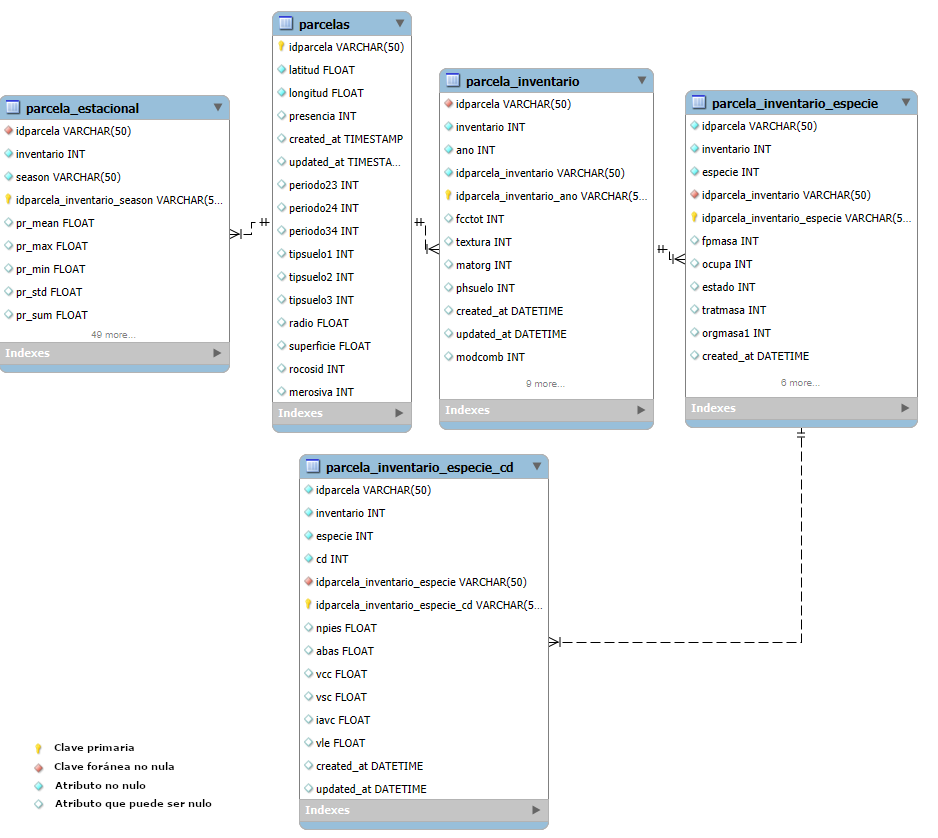
\includegraphics[width=1\linewidth]{figuras/estructura_base_datos_informe_con_leyenda.png}
    \caption{Estructura de la base de datos}
    \label{fig:estructura_ddbb}
\end{figure}


\begin{table}[H]
\renewcommand{\arraystretch}{2.2}
\setlength{\tabcolsep}{5pt}
\centering
\resizebox{\textwidth}{!}{%
\begin{tabular}{|>{\centering\arraybackslash}m{4cm}|>{\centering\arraybackslash}m{3cm}|m{8cm}|}
\hline
\multicolumn{3}{|c|}{\cellcolor[HTML]{D9EAD3}\textbf{\color[HTML]{000000}parcelas: identificación, localización y caracterización básica de las parcelas forestales}} \\
\hline
\cellcolor[HTML]{D9EAD3}\textbf{\color[HTML]{000000}Variable} &
\cellcolor[HTML]{D9EAD3}\textbf{\color[HTML]{000000}Tipo} &
\cellcolor[HTML]{D9EAD3}\textbf{\color[HTML]{000000}Descripción}  \\
\hline
\textbf{idparcela} & varchar(50) & Identificador único de la parcela \\
\hline
latitud & float & Coordenada de latitud de la parcela \\
\hline
longitud & float & Coordenada de longitud de la parcela \\
\hline
%presencia & int & Indica presencia de la parcela en los distintos inventarios (Anexo \ref{anexo:presencia}) \\
%\hline
created\_at & timestamp & Fecha de creación del registro \\
\hline
updated\_at & timestamp & Fecha de última modificación del registro \\
\hline
ele\_values & float & Altura de la parcela desde el nivel del mar \\
\hline
asp\_values & float & Orientación de la parcela en grados \\
\hline
slo\_values & float & Pendiente del terreno de la parcela \\
\hline
periodo23 & int & Años transcurridos entre el apeo de la parcela en el IFN2 y el apeo en el IFN3 \\
\hline
periodo24 & int & Años transcurridos entre el apeo de la parcela en el IFN2 y el apeo en el IFN4 \\
\hline
periodo34 & int & Años transcurridos entre el apeo de la parcela en el IFN3 y el apeo en el IFN3 \\
\hline
tipsuelo1, tipsuelo2, tipsuelo3 & int & Tipos de suelo identificados en la parcela (diferentes categorías o clases) \\
\hline
radio & float & Estimación del radio circular de la parcela (m)\\
\hline
superficie & float & Estimación de la superficie circular de la parcela ($m^2$) \\
\hline
rocosid & int & Grado de rocosidad del terreno \\
\hline
merosiva & int & Manifestaciones erosivas observadas en la parcela \\
\hline
\end{tabular}%
}
\caption{Estructura de la tabla \texttt{parcelas}. Contiene información general, geográfica y edáfica de cada unidad de muestreo en la base de datos. Se pueden consultar las claves de las variables en los anexos.}
\label{tab:parcela1}
\end{table}



\begin{table}[H]
\renewcommand{\arraystretch}{2.2}
\setlength{\tabcolsep}{5pt}
\centering
\resizebox{\textwidth}{!}{%
\begin{tabular}{|>{\centering\arraybackslash}m{5cm}|>{\centering\arraybackslash}m{3cm}|m{9cm}|}
\hline
\multicolumn{3}{|c|}{\cellcolor[HTML]{D9EAD3}\textbf{\color[HTML]{000000}parcela\_inventario: registros asociados a cada parcela para los inventarios IFN2, IFN3 e IFN4}} \\
\hline
\cellcolor[HTML]{D9EAD3}\textbf{Campo} &
\cellcolor[HTML]{D9EAD3}\textbf{Tipo} &
\cellcolor[HTML]{D9EAD3}\textbf{Descripción} \\
\hline
idparcela\_inventario\_ano & varchar(50) & Identificador único por parcela y año \\
\hline
\textbf{idparcela\_inventario} & varchar(50) & Identificador del inventario de la parcela \\
\hline
idparcela & varchar(50) & Identificador de la parcela \\
\hline
inventario & int & Número del inventario (2, 3 o 4) \\
\hline
ano & int & Año de apeo de la parcela e inventario \\
\hline
fcctot & int & Fracción de cabida cubierta total en la parcela e inventario\\
\hline
textura & int & Textura del suelo en la parcela e inventario\\
\hline
matorg & int & Contenido de materia orgánica en la parcela e inventario\\
\hline
phsuelo & int & pH del suelo en la parcela e inventario\\
\hline
modcomb & int & Modelo de combustible en la parcela e inventario\\
\hline
espcmue & int & Espesor de capa muerta en la parcela e inventario\\
\hline
fccarb & int & Fracción cubierta arbórea en la parcela e inventario\\
\hline
disesp & int & Distribución espacial de las especies en la parcela e inventario\\
\hline
comesp & int & Composición de las especies en la parcela e inventario\\
\hline
%suelo & int & Variable creada por clustering con las caracteristicas del suelo\\
%\hline
clasuelo & int & Clase del suelo (ifn2)\\
\hline
created\_at & datetime & Fecha de creación del registro \\
\hline
updated\_at & datetime & Fecha de última modificación del registro \\
\hline
\end{tabular}%
}
\caption{Estructura de la tabla \texttt{parcela\_inventario}. Contiene los registros asociados a cada parcela en cada inventario (IFN2, IFN3, IFN4).}
\label{tab:parcela_inventario1}
\end{table}


\begin{table}[H]
\renewcommand{\arraystretch}{2.2}
\setlength{\tabcolsep}{5pt}
\centering
\resizebox{\textwidth}{!}{%
\begin{tabular}{|>{\centering\arraybackslash}m{5cm}|>{\centering\arraybackslash}m{3cm}|m{9.5cm}|}
\hline
\multicolumn{3}{|c|}{\cellcolor[HTML]{D9EAD3}\textbf{\color[HTML]{000000}parcela\_inventario\_especie: información por especie forestal presente en cada parcela e inventario}} \\
\hline
\cellcolor[HTML]{D9EAD3}\textbf{Campo} &
\cellcolor[HTML]{D9EAD3}\textbf{Tipo} &
\cellcolor[HTML]{D9EAD3}\textbf{Descripción} \\
\hline
idparcela & varchar(50) & Identificador de la parcela \\
\hline
inventario & int & Número del inventario (2, 3 o 4) \\
\hline
especie & int & Código de la especie forestal \\
\hline
idparcela\_inventario & varchar(50) & Identificador del inventario de la parcela \\
\hline
\textbf{idparcela\_inventario\_especie} & varchar(50) & Identificador único por parcela, inventario y especie \\
\hline
fpmasa & int & Forma principal de la masa formada por la especie en la parcela e inventario\\
\hline
ocupa & int & Ocupación de la especie en la parcela e inventario\\
\hline
estado & int & Estado general de la masa formada por la especie en la parcela e inventario\\
\hline
tratmasa & int & Tipo de tratamiento aplicado a la masa formada por la especie en la parcela e inventario\\
\hline
orgmasa1 & int & Origen principal de la masa formada por la especie en la parcela e inventario\\
\hline
masa & int & Tipo de masa forestal (ifn2)\\
\hline
origen & int & Origen de la masa formada por la especie en la parcela e inventario\\
\hline
ca & float & Carbono aéreo capturado por la especie en la parcela e inventario (t/ha)\\
\hline
cr & float & Carbono radical capturado por la especie en la parcela e inventario (t/ha)\\
\hline
c & float & Carbono total capturado por la especie en la parcela e inventario (t/ha)\\
\hline
created\_at & datetime & Fecha de creación del registro \\
\hline
updated\_at & datetime & Fecha de última modificación del registro \\
\hline
\end{tabular}%
}
\caption{Estructura de la tabla \texttt{parcela\_inventario\_especie}. Contiene información por especie forestal presente en cada parcela en cada inventario.}
\label{tab:parcela_inventario_especie1}
\end{table}



\begin{table}[H]
\renewcommand{\arraystretch}{2.2}
\setlength{\tabcolsep}{5pt}
\centering
\resizebox{\textwidth}{!}{%
\begin{tabular}{|>{\centering\arraybackslash}m{6cm}|>{\centering\arraybackslash}m{3cm}|m{8.5cm}|}
\hline
\multicolumn{3}{|c|}{\cellcolor[HTML]{D9EAD3}\textbf{\color[HTML]{000000}parcela\_inventario\_especie\_cd: información por clase diamétrica para cada especie en cada parcela}} \\
\hline
\cellcolor[HTML]{D9EAD3}\textbf{Campo} &
\cellcolor[HTML]{D9EAD3}\textbf{Tipo} &
\cellcolor[HTML]{D9EAD3}\textbf{Descripción} \\
\hline
cd & int & Clase diamétrica del conjunto de árboles estudiado \\
\hline
idparcela\_inventario\_especie & varchar(50) & ID de especie por parcela e inventario \\
\hline
\textbf{idparcela\_inventario\_especie\_cd} & varchar(50) & Identificador único del registro \\
\hline
npies & float & Número de pies de la clase diamétrica y especie en la parcela e inventario \\
\hline
abas & float & Área basal total del conjunto de árboles de la clase diamétrica y especie en la parcela e inventario \\
\hline
vcc & float & Volumen con corteza del conjunto de árboles de la clase diamétrica y especie en la parcela e inventario\\
\hline
vsc & float & Volumen sin corteza del conjunto de árboles de la clase diamétrica y especie en la parcela e inventario\\
\hline
iavc & float & Incremento anual del volumen con corteza del conjunto de árboles de la clase diamétrica y especie en la parcela e inventario\\
\hline
vle & float & Volumen de leñas del conjunto de árboles de la clase diamétrica y especie en la parcela e inventario\\
\hline
created\_at & datetime & Fecha de creación del registro \\
\hline
updated\_at & datetime & Fecha de última modificación del registro \\
\hline
\end{tabular}%
}
\caption{Estructura de la tabla \texttt{parcela\_inventario\_especie\_cd}. Incluye información por clase diamétrica (CD) para cada especie presente en una parcela.}
\label{tab:parcela_inventario_especie_cd1}
\end{table}




\begin{table}[H]
\renewcommand{\arraystretch}{2.2}
\setlength{\tabcolsep}{5pt}
\centering
\resizebox{\textwidth}{!}{%
\begin{tabular}{|>{\centering\arraybackslash}m{5cm}|>{\centering\arraybackslash}m{3cm}|m{9.5cm}|}
\hline
\multicolumn{3}{|c|}{\cellcolor[HTML]{D9EAD3}\textbf{\color[HTML]{000000}parcela\_inventario\_estacion: métricas climáticas y espectrales por estación e inventario}} \\
\hline
\cellcolor[HTML]{D9EAD3}\textbf{Campo} &
\cellcolor[HTML]{D9EAD3}\textbf{Tipo} &
\cellcolor[HTML]{D9EAD3}\textbf{Descripción} \\
\hline
\textbf{idparcela\_inventario\_season} & varchar(50) & Identificador único por parcela e inventario por estación \\
\hline
idparcela & varchar(50) & Identificador de la parcela \\
\hline
inventario & int & Número del inventario (2, 3 o 4) \\
\hline
season & varchar(50) & Estación del año (e.g., invierno, primavera) \\
\hline
pr\_mean, sum, max, min, std  & float & Estadísticos de precipitación \\
\hline
t2m\_mean, max, min, std & float & Estadísticos de temperatura del aire a 2m del suelo\\
\hline
skt\_mean, max, min, std & float & Estadísticos de temperatura de la superficie del suelo \\
\hline
stl1\ – \ stl4\_mean, max, min, std & float & Estadísticos de temperatura en 4 capas del subsuelo \\
\hline
evi-gndvi-ndii-ndvi\_mean, max, min, std & float & Estadísticos de índices espectrales \\
\hline
created\_at & datetime & Fecha de creación del registro \\
\hline
updated\_at & datetime & Fecha de última modificación del registro \\
\hline
\end{tabular}%
}
\caption{Estructura de la tabla \texttt{parcela\_inventario\_estacion}. Contiene métricas climáticas y espectrales agregadas estacionalmente para cada parcela e inventario.}
\label{tab:parcela_estacional1}
\end{table}
